\addbibresource{reference.bib}

\chapter{Polovodičové pixelové detektory ionizujícího záření}\label{det}
Ionizující záření je lidskými smysly nedetekovatelné. Jeho schopnost ionizovat svoji energií látku, dala vzniku detekční technice a metod toto záření měřit. Tato kapitola bude věnována zatím nejpokročilejší instrumentaci pro detekci ionizujícího záření a jeho charakteristických vlastností - hybridním polovodičovým pixelovým detektorům.

Existuje celá řada částicových pixelových detektorů (CMS pixel detector, Pilatus apod.), v této práci však budou zmíněny jen detektory z rodiny Medipix, které jsou vyvíjeny v rámci stejnojmenné kolaborace Medipix\footnote{\url{http://medipix.web.cern.ch/}} v CERN. Tato kolaborace sdružuje několik desítek vědeckých institucí a univerzit po celém světe, mezi které patří od roku 1999 i ÚTEF ČVUT v Praze.

\begin{figure}[th!]
	\begin{center}
		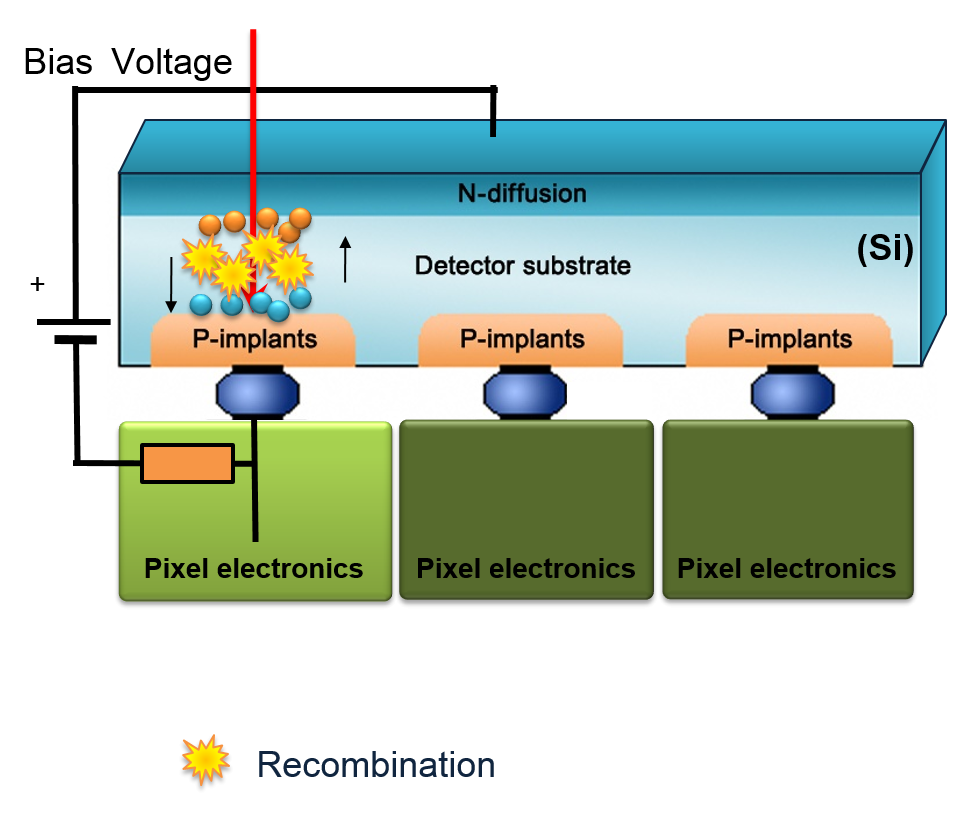
\includegraphics[width=8.5cm]{figures/det_recombination.png}
		\caption{Princip detekce ionizujícího záření (převzato z \cite{PlatkevicDisertace})}
		\label{fig:det:recomb}
	\end{center}
\end{figure}

%********************************************************************************
% Princip detekce
%********************************************************************************
\section{Princip detekce}
Činnost těchto detektorů je založena na známém principu detekce ionizujícího záření v polovodiči. 

Na obrázku \ref{fig:det:recomb} je znázorněn princip této detekce. V horní části se nachází polovodičový senzor, pro který je jako materiál nejčastěji použit křemík, ale výjimkou není také \texttt{GaAs}, či \texttt{CdTe}. Pod tímto senzorem se nachází vyčítací elektronika, která tvoří jednotlivé pixely. Jako náhradní schéma tohoto obvodu si můžeme představit diodu zapojenou v závěrném směru, skrze kterou protéká jen minimální proud. Vnikne-li ale do polovodičového senzoru ionizovaná částice, která v senzoru zanechá jisté množství své deponované energie, dojde ke vzniku elektron-děrových párů a díky lavinovému jevu i k následnému otevření PN přechodu. Tím dojde k vyvolání proudového pulsu, které je pomocí měřícího odporu převeden na napětí, které je dále měřící elektronikou zpracováváno.

\begin{figure}[th]
	\begin{center}
		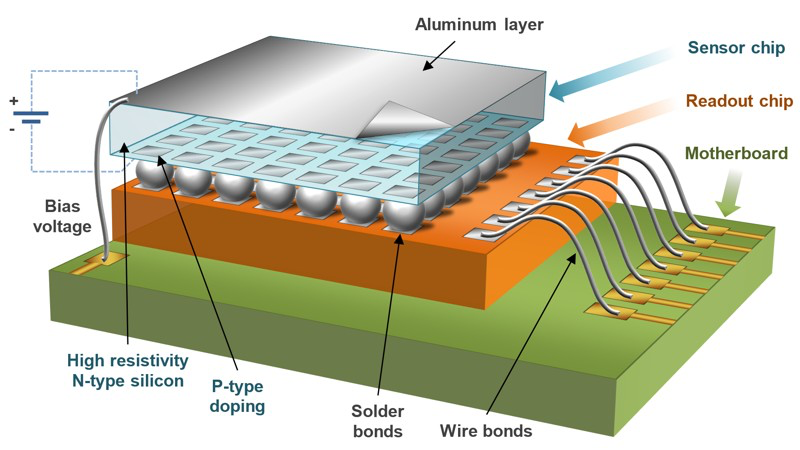
\includegraphics[width=12cm]{figures/det_chip.png}
		\caption{Struktura hybridního polovodičového pixelového detektoru (převzato z \cite{PlatkevicDisertace})}
		\label{fig:det:chip}
	\end{center}
\end{figure}

Na obrázku \ref{fig:det:chip} je znázorněna struktura tohoto detektoru. Nahoře se nachází, již výše zmíněný, polovodičový senzor, který je spojen s integrovaným \texttt{ASIC}\footnote{z angl. Application Specific Integrated Circuit} vyčítacím čipem (tzv. \texttt{Readout chip}) pomocí technologie zvané \texttt{bump-bonding}. Odtud také pochází název "hybridní" - jedná se spojení senzoru a \texttt{ASIC} čipu. Každý pixel tedy tvoří jeden PN přechod. Vyčítací čip je dále spojen s další nezbytnou elektronikou (na obr \ref{fig:det:chip} znázorněnou jako \texttt{Motherboard}) pomocí tzv. \texttt{wire-bonds}. Z této elektroniky je dále vyvedeno napětí na polovodičový senzor - \texttt{bias}.

%********************************************************************************
% Medipix detektory
%********************************************************************************
\section{Detektory rodiny Medipix}\label{det:med}
Mezi mezi nejznámější detektory rodiny Medipix patří: Medipix1, Medipix2 \cite{Llopart-medipix2}, Timepix \cite{Llopart2008106}, Medipix3, nově Timepix3 \cite{timepix3} a v průběhu příštího roku k nim přibude i Timepix2. 

\begin{description}
	\item[Medipix1] Medipix1 byl prvním detektorem z této rodiny a byl uvedený v roce 1997. Také je známy pod názvem PCC (z angl. Photon Counting Chip). Jednalo se o prototyp digitálního \texttt{CMOS}\footnote{z angl. Complementary Metal–Oxide–Semiconductor} zobrazovacího čipu, který našel uplatnění ve vysokoenergetických fyzikálních experimentech \cite{medipix-www} a byl schopný operovat jen v \texttt{Medipix módu} (viz \ref{det:mod}). Tento detektor měl matici $64\times64$ pixelů, každý s hranou o délce $170~\mu m$ a celková aktivní plocha byla $1,2~cm^2$. Detektor obsahoval $15$-bitový čítač, kterým byl schopen v rámci jedné akvizice zaregistrovat až $32767$ událostí.

	\item[Medipix2] Medipix2 je přímým následníkem Medipix1. Tento model především profitoval z rychlého pokroku \texttt{CMOS} technologie, díky kterému bylo možné přidání nové funkcionality a především zmenšení velikosti pixelů. Detektor obsahoval matici $256\times256$ pixelů, délka hrany jednoho pixelu se zmenšila na $55~\mu m$ a celková aktivní plocha vzrostla na $2~cm^2$.

	\item[Timepix]\label{det:tim} Tento detektor vychází z detektoru Medipix2, prodělal však výraznou obměnu digitální části. Byla přidána synchronizační logika, která přinesla dva nové módy - TOT (měření energie) a TOA (měření doby příletu částice), přičemž každý pixel v jeden okamžik umožňuje měřit jen v jednom módu
	(vice o módech bude zmíněno v \ref{det:mod}). Další možností je nastavení globálního tresholdu\footnote{Treshold je úroveň komparačního napětí, které je porovnáváno s aktuálním měřícím napětím na každém pixelu. Je-li tato úroveň překročena, dojde k detekováni události.} s lokální úpravou pro jednotlivé pixely o $4 b$. 

	\item[Medipix3] U Medipix3, jehož předchůdce byl Medipix2, byla výrazným způsobem přepracována vyčítací elektronika za cílem snížení zkreslení, způsobeném sdílením náboje mezi sousedními pixely (tento efent je také znám pod pojmem \texttt{Charge Sharing} efekt \cite{Jakubek-radiography_and_charge_sharing}). 

	\begin{figure}[th]
	\begin{center}
		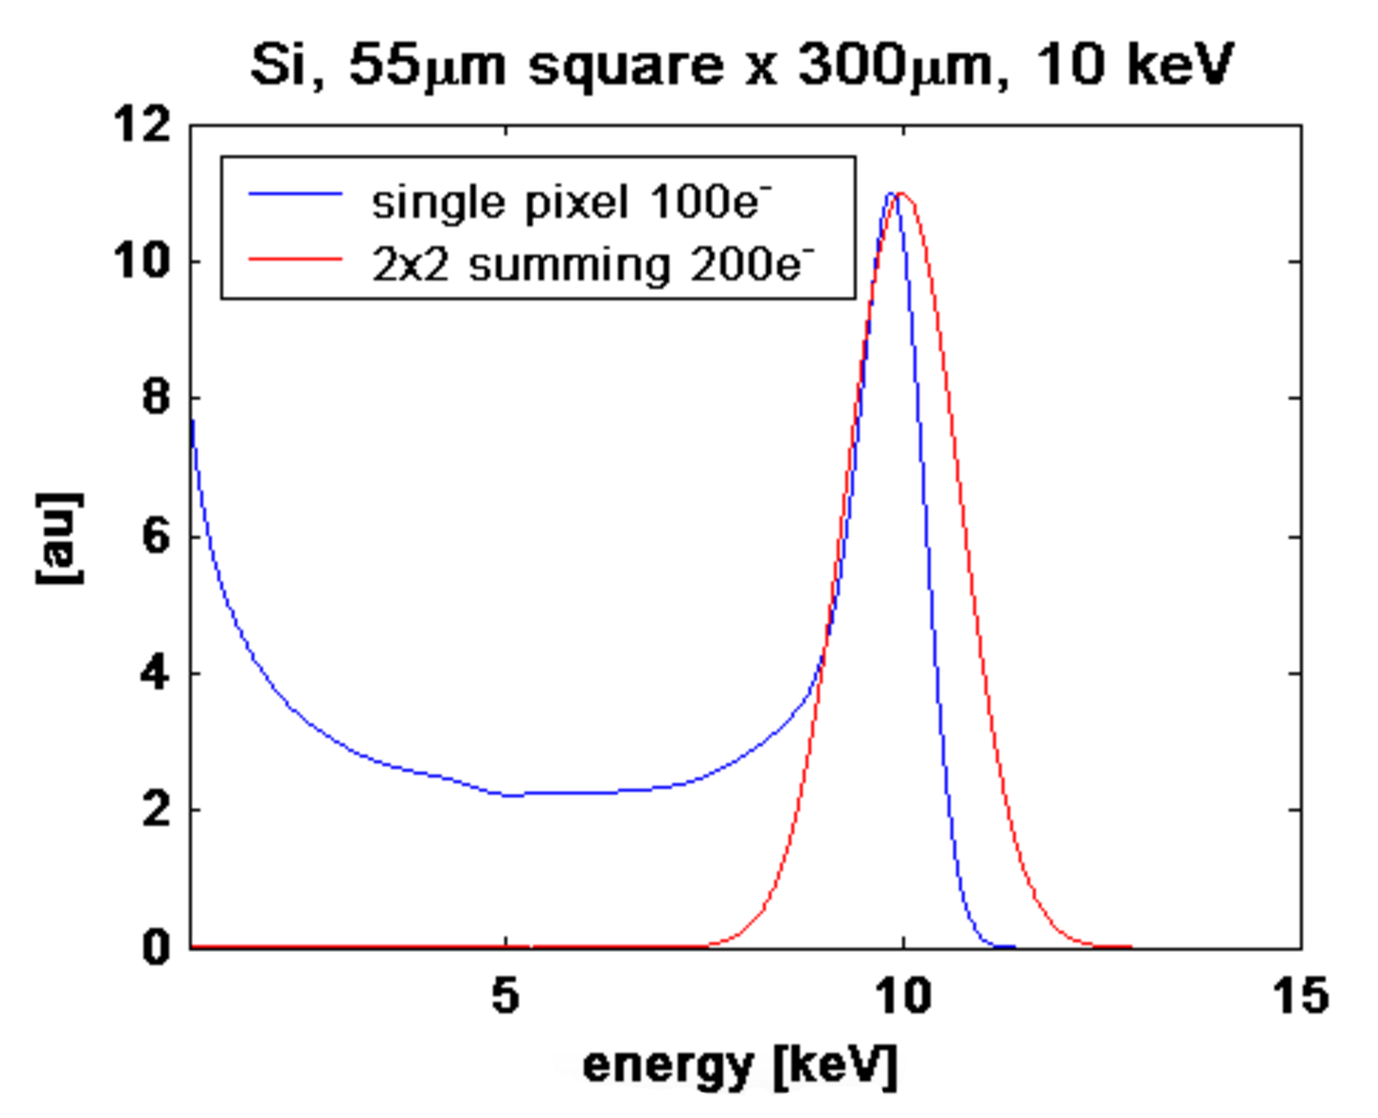
\includegraphics[width=8cm]{figures/det_charge_sharing.png}
		\caption{Charge Sharing Efekt (převzato z \cite{medipix-www})}
		\label{fig:det:charge_sharing}
	\end{center}
	\end{figure}

	Když dopadne nabitá částice na polovodičový senzor, vzniknou elektron-děrové páry, které jsou staženy nejen zasaženým pixelem, ale vetšinou i několika sousedními. To samo o sobě je žádoucí jev, problém ale nastává, když vyčtená energie sousedními pixely je nižší, než jejich prahová, potom dochází ke, již výše zmíněnému, zkreslení. 
	
	Obrázek \ref{fig:det:charge_sharing} je demonstrací tohoto jevu. Zobrazuje histogram detekovaných energií pro jeden pixel. Když každý pixel operuje zcela nezávisle (na obrázku modře), je patrné, že daný pixel registroval i události sousedních pixelů, vzniklé \texttt{Charge Sharing} efektem. Tento problém odstraňuje \texttt{CSM} \ref{det:mod:csm} mód a především možnost vyčítat jednotlivé události (nikoliv až celé snímky), což také odstraňuje mrtvou dobu detektoru. \texttt{CSM} mód přičte k energii zasaženého pixelu i energii sousedních pixelů - viz obr. \ref{fig:det:charge_sharing} červeně.

	\item[Timepix3] Nejnovějším přírůstkem této rodiny detektorů je Timepix3. Oproti svému předchůdci Timepix má tento detektor vylepšenou vyčítací logiku a o jeden čítač více. To mu mimo jiné umožňuje měřit v TOT a TOA módu současně. Navíc ještě přináší \texttt{Data-driven} vyčítací mód (obdobně, jako Medipix3), který na rozdíl od \texttt{Frame-based} vyčítání odstraňuje mrtvou dobu detektoru.

\end{description}

%********************************************************************************
% Módy detektorů
%********************************************************************************
\section{Módy detektorů}\label{det:mod}
V této podkapitole budou popsány všechny nejpoužívanější módy detektorů z rodiny Medipix. 
Na obrázku \ref{fig:det:signal_proc} jsou znázorněny tři pixely detektoru s blokovým schématem vyčítací elektroniky. Jak již bylo zmíněno výše, interagující částice s polovodičovým povrchem detektoru vyvolá proudový pulz. Ten je měřícím odporem převeden na napětí, které je dále zesilovačem zesíleno (na obr. \ref{fig:det:signal_proc} jako \texttt{Amplifier}). Toto napětí je dále porovnáno komparátorem s komparačním napětím (tzv. tresholdem), jak je znázorněno na obr. \ref{fig:det:signal_proc}. S informací z tohoto komparátoru je dále naloženo dle módu detektoru. Pro úplnost je třeba dodat, že \texttt{Shutter} na obr. \ref{fig:det:signal_proc} slouží pro spouštění, resp. ukončování akvizice.

\begin{figure}[th!]
	\begin{center}
		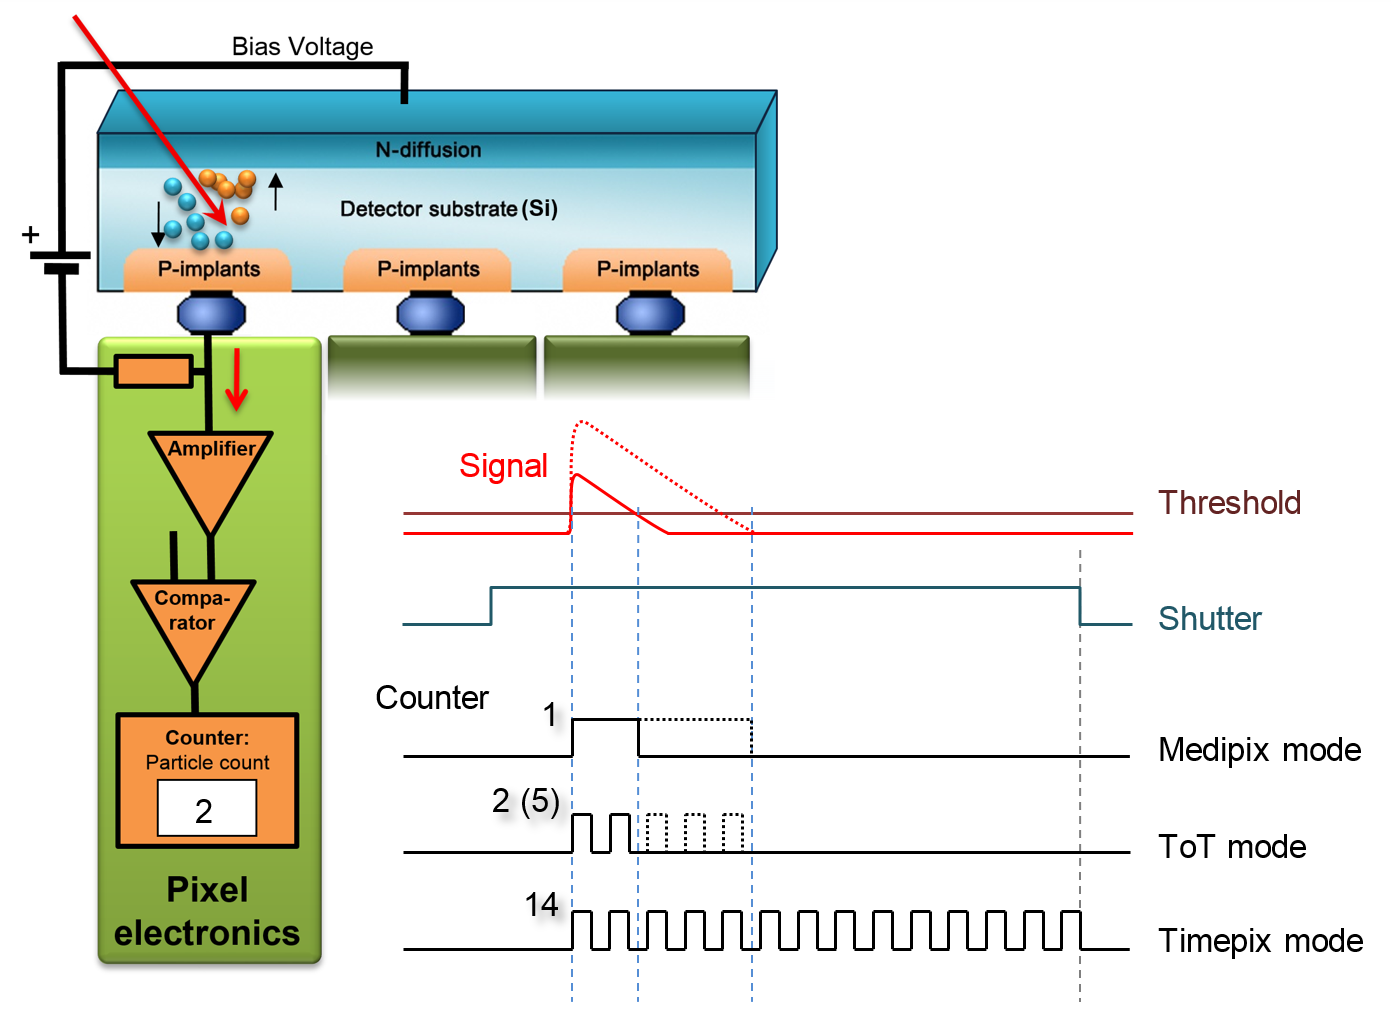
\includegraphics[width=10.75cm]{figures/det_pix.png}
		\caption{Zpracování signálu z pohledu módu pixelu (převzato z \cite{PlatkevicDisertace})}
		\label{fig:det:signal_proc}
	\end{center}
\end{figure}

\begin{description}
	\item[Medipix mód] Tento mód počítá počet částic, které během doby akvizice dopadly na aktivní plochu detektoru. Na obrázku \ref{fig:det:signal_proc} znázorněn, jako \texttt{Medipix mode}.
	\item[TOT (Time-Over-Treshold)] Tento mód udává, jak dlouhou dobu (v počtu hodinových cyklů měřící frekvence) bylo zesílené napětí na detektoru vyšší, než komparační (treshold). Počet těchto cyklů je zhruba ekvivalentní energii deponované částice, ale jelikož každý pixel má jiné elektronické vlastnosti, je třeba pro získání energie z TOT detektor kalibrovat - o tom pojednává kapitola \ref{calib}. Tento mód je podporovaný všemi Timepix detektory (ze zde uvedených detektorů).
	\item[TOA (Time-Of-Arrival)] Pixel v tomto módu spustí svůj čítač po překročení tresholdu, čily vůči akvizičnímu času udává čas příletu částice. Tento mód je také známý pod označením \texttt{Timepix mode} a nalézá své uplatnění především při měření koincidencí (rekonstrukce trajektorie částice, interagující s více detektory pomocí času dopadu a souřadnic zasažených pixelů). Tento mód je podporovaný všemi Timepix detektory (ze zde uvedených detektorů).
	\item[SPM (Single Pixel Mode)] V tomto módu každý pixel operuje zcela samostatně a to v Medipix módu.
	\item[CSM (Charge Summing Mode)]\label{det:mod:csm} Tento mód odstraňuje zkreslení vzniklé \texttt{Charge Sharing} efektem pomocí přičtení energie do zasaženého pixelu z pixelů okolních. Jako zasažený pixel se určí pixel s nejvyšší energií. Tento mód podporuje jen Medipix3 (ze zde uvedených detektorů).

\end{description}

%********************************************************************************
% FITPix
%********************************************************************************
\section{FITPix}\label{det:fitpix}

\begin{figure}[th!]
	\begin{center}
		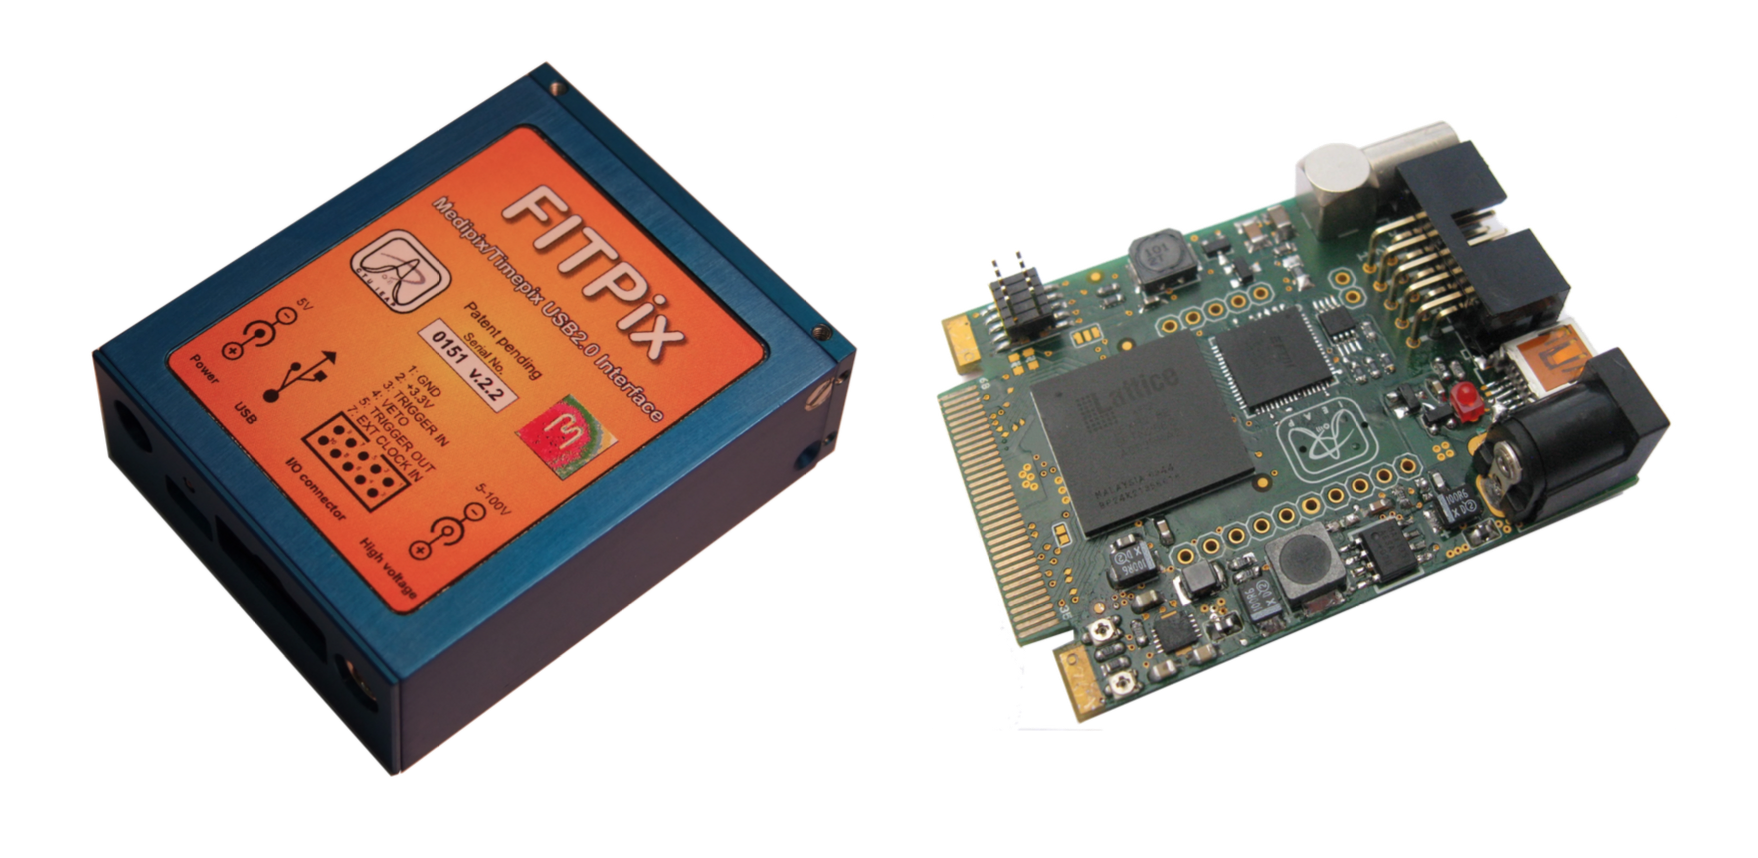
\includegraphics[width=11cm]{figures/fitpix.png}
		\caption{FITPix}
		\label{fig:det:fitpix}
	\end{center}
\end{figure}

FITPix\footnote{z angl. Fast Interface for Timepix Pixel Detectors} \cite{fitpix} je vyčítací rozhraní, pracující téměř se všemi detektory rodiny Medipix, vyvíjené v ÚTEF ČVUT v Praze od roku 2010 - viz obr. \ref{fig:det:fitpix}. Toto rozhraní se skládá z FPGA\footnote{z angl. Feld Programmable Gate Array} obvodu, USB 2.0 rozhraní, DAC převodníků (převodník digitálního signálu na analogový), ADC převodníků (převodník analogového signálu na digitální) a z obvodů generující napětí pro polovodičový senzor (tzv. bias). Toto zařízení umožňuje plnohodnotné ovládání připojeného detekčního čipu, včetně nastavování měřící frekvence, tresholdu, řízení shutteru (sloužícího pro ovládání akvizice, viz \ref{det:mod}) apod. Také přináší možnost ovládat shutter pomocí hardwarového trigger signálu pro měření s více detektory současně, resp. pro jejich synchronizaci.

Tato architektura s FPGA byla použita především z důvodu dosažení vyšších datových toků a také vyšší radiační odolnosti, které by za použití konvenčních mikroprocesorů nemohlo být dosaženo. Další výhodou je menší počet aktivních prvků, což se projeví krom spotřeby i na nižších tepelných ztrátách. Tento parametr je velice důležitý, především pro nasazení ve vakuu.

%********************************************************************************
% Pixelman
%********************************************************************************
\section{Pixelman}\label{det:pixelman}
Pixelman \cite{pixelman} je softwarový balík, vyvíjený v ÚTEF ČVUT v Praze, sloužící pro řízení detektorů z rodiny Medipix pomocí vyčítacího rozhraní FITPix \ref{det:fitpix}. Tento software umožňuje akvizici dat, jejich vizualizaci a následnou analýzu.

Jedná se o vysoce modulární systém, který mimo jiné umožňuje rozšíření své funkcionality o pluginy, které mají přístup k funkcím, poskytovaným jádrem Pixelmanu. Dokonce každý plugin může zaregistrovat své funkce, takže i ostatní pluiny mohou využívat jeho funkcionalitu. Jsou podporovány pluginy, vyvinuté v jazycích Java, C/C++ a Python. Na obrázku \ref{fig:det:pixelman} je znázorněna softwarová architektura Pixelmana.

\begin{figure}[th!]
	\begin{center}
		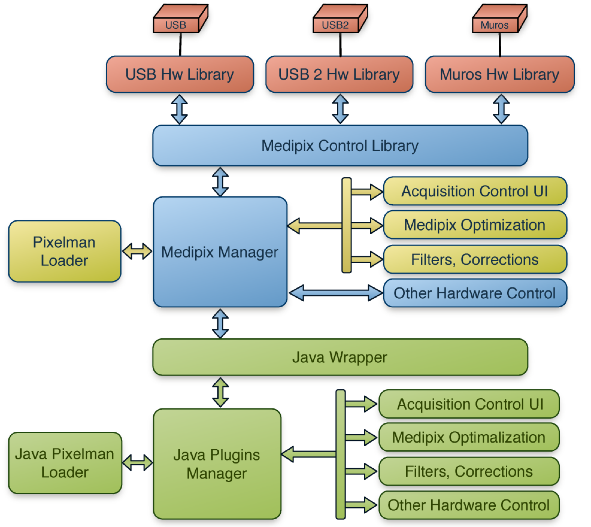
\includegraphics[width=10.25cm]{figures/pixelman.png}
		\caption{Pixelman - sw architektura (převzato z \cite{pixelman})}
		\label{fig:det:pixelman}
	\end{center}
\end{figure}


%********************************************************************************
% Aplikace
%********************************************************************************
%\section{Aplikace}








